% The generic preamble
\documentclass[10pt,letterpaper,fleqn,titlepage]{article}

% Define packages to use
\usepackage{natbib}
\usepackage[dvips]{graphicx,color}
\usepackage{amsmath,amssymb}
\usepackage{bm}
\usepackage{caption}
\usepackage{xr}
\usepackage{ifthen}
\usepackage[dvipdfm,colorlinks,linkcolor=blue,citecolor=blue,urlcolor=blue]{hyperref}
\usepackage{fancybox}
\usepackage{textcomp}
\usepackage{alltt}
%\usepackage{floatflt}
%\usepackage{svn}


% Redefine default page
\setlength{\textheight}{9in}  % 1" above and below
\setlength{\textwidth}{6.75in}   % 0.5" left and right
\setlength{\oddsidemargin}{-0.25in}

% Redefine default paragraph
\setlength{\parindent}{0pt}
\setlength{\parskip}{1ex plus 0.5ex minus 0.2ex}

% Define caption width and default fonts
\setlength{\captionmargin}{0.5in}
\renewcommand{\captionfont}{\sffamily}
\renewcommand{\captionlabelfont}{\bfseries\sffamily}

% Define commands for super- and subscript in text mode
\newcommand{\superscript}[1]{\ensuremath{^\textrm{#1}}}
\newcommand{\subscript}[1]{\ensuremath{_\textrm{#1}}}

% Derived commands
\newcommand{\invcm}{\textrm{cm\superscript{-1}}}
\newcommand{\micron}{\ensuremath{\mu\textrm{m}}}

\newcommand{\df}{\ensuremath{\delta f}}
\newcommand{\Df}{\ensuremath{\Delta f}}
\newcommand{\dx}{\ensuremath{\delta x}}
\newcommand{\Dx}{\ensuremath{X_{max}}}
\newcommand{\Xeff}{\ensuremath{X_{eff}}}

\newcommand{\water}{\textrm{H\subscript{2}O}}
\newcommand{\carbondioxide}{\textrm{CO\subscript{2}}}
\newcommand{\ozone}{\textrm{O\subscript{3}}}

\newcommand{\taup}[1]{\ensuremath{\tau_{#1}}}
\newcommand{\efftaup}[1]{\ensuremath{\tau_{#1}^{*}}}

\newcommand{\textbfm}[1]{\boldmath\ensuremath{#1}\unboldmath}

\newcommand{\rb}[1]{\raisebox{1.5ex}[0pt]{#1}}

\newcommand{\f}[1]{\texttt{#1}}

% Define how equations are numbered
\numberwithin{equation}{section}
\numberwithin{figure}{section}
\numberwithin{table}{section}

% Define a command for title page author email footnote
\newcommand{\email}[1]
{%
  \renewcommand{\thefootnote}{\alph{footnote}}%
  \footnote{#1}
  \renewcommand{\thefootnote}{\arabic{footnote}}
}

% Define a command to print the Office Note subheading
\newcommand{\notesubheading}[1]
{%
  \ifthenelse{\equal{#1}{}}{}
  { {\Large\bfseries Office Note #1\par}%
    {\scriptsize \sc This is an unreviewed manuscript, primarily intended for informal}\\ 
    {\scriptsize \sc exchange of information among JCSDA researchers\par}%
  }
}

% Redefine the maketitle macro
\makeatletter
\def\docseries#1{\def\@docseries{#1}}
\def\docnumber#1{\def\@docnumber{#1}}
\renewcommand{\maketitle}
{%
  \thispagestyle{empty}
  \vspace*{1in}
  \begin{center}%
     \sffamily
     {\huge\bfseries Joint Center for Satellite Data Assimilation\par}%
     \notesubheading{\@docnumber}
  \end{center}
  \begin{flushleft}%
     \sffamily
     \vspace*{0.5in}
     {\Large\bfseries\ifthenelse{\equal{\@docseries}{}}{}{\@docseries: }\@title\par}%
     \medskip
     {\large\@author\par}%
     \medskip
     {\large\@date\par}%
     \bigskip\hrule\vspace*{2pc}%
  \end{flushleft}%
  \newpage
  \setcounter{footnote}{0}
}
\makeatother
\docseries{}
\docnumber{}


% Define a command for a DRAFT watermark
\usepackage{eso-pic}
\newcommand{\draftwatermark}
{
  \AddToShipoutPicture{%
    \definecolor{lightgray}{gray}{.85}
    \setlength{\unitlength}{1in}
    \put(2.5,3.5){%
      \rotatebox{45}{%
        \resizebox{4in}{1in}{%
          \textsf{\textcolor{lightgray}{DRAFT}}
        }
      }
    }
  }
}




% Derived commands
\newcommand{\microtesla}{\ensuremath{\mu\textrm{T}}}
\newcommand{\degree}{\ensuremath{^\circ}}

% Title info
\title{Model Intercomparisons with LBLDIS and LBLDIS Components}
\author{David Neil Groff\email{david.groff@noaa.gov}\\JCSDA/EMC/SAIC\\[0.25in]
        Paul van Delst\email{paul.vandelst@noaa.gov}\\JCSDA/EMC/SAIC\\[0.25in]}
\date{April, 2008}
\docnumber{??}
\docseries{CRTM}


%-------------------------------------------------------------------------------
%                            Ze document begins...
%-------------------------------------------------------------------------------
\begin{document}
\maketitle

\begin{abstract}
This report discusses work that has been done to compare CRTM and LBLDIS components for clear and cloudy sky conditions. The proceedures used for running LBLDIS and performing the comparisons are described. Furthermore, systematic errors associated with these proceedures are described and quantified.
The components of the LBLDIS model will be used as references for validating the CRTM's handling of gas absorption and cloud scattering, and solver of the radiative transfer equation.   
   

\textbf{Keywords}: CRTM, LBLRTM, LBLDIS, Clouds  
\end{abstract}

\section{Running LBLDIS}
%=================
LBLDIS is a radiative transfer model that combines AER's line by line radiative transfer model (LBLRTM) and the discrete ordinate radiative transfer model (DISORT) and is able to compute radiances
for scattering atmospheres. The LBLDIS model requires the following inputs: LBLDIS formatted parameter files, 
LBLRTM optical depth output, and the atmospheric layering and structure information used by the 
LBLRTM. A further description of these inputs are provided in the following subsections.

\subsection{LBLRTM Calculations}
The LBLRTM performs gas absorption computations and is run externally to LBLDIS.
To run the LBLRTM it is necessary to first create TAPE5 files that specify the level quantities
of the profile data to be used for running the LBLRTM. In this project CRTM atmosphere layer data was converted to level data in
order to create TAPE5 files. Linear extrapolation is performed to obtain the surface level quantities 

\begin{equation}
level(1) = layer(1) - ((layer(2) - layer(1))/2)
\end{equation}          

and a simple averaging scheme is used to obtain the level quantities from level k=2 to the top of the atmosphere. 

\begin{equation}
level(k) = (layer(k) + layer(k+1)/2)
\end{equation}

The LBLRTM calculates layer atmosphere quantities using the level atmosphere quantities provided in the TAPE5 files. The LBLRTM calculated layer atmosphere quantities are included in TAPE7 files and are used by the LBLRTM to perform the gas computations.
In addition to providing the level profile quantities the TAPE5 file is used to specify the wavenumber (cm\superscript{-1}) range and view geometry for the LBLRTM calculations. For the initial results presented in this report the wavenumber range specifications have been set to span the spectral response functions for hirs4\textunderscore{}n18 channels 1-19 and the view geometry has been set to nadir. To correctly account for gas absorption away from absorption lines the continuum option field must be set to 1 in the TAPE5 files. The LBLRTM is run at single precision for compatability with LBLDIS.

\subsection{LBLDIS Parameter Files}
Parameter files needed to run the LBLDIS provide the cloud data, surface data, view geometry, wavenumber specifications (range and spacing), a path to cloud optical property look up table (LUT) data and a path to the LBLRTM output data. For accurate comparisons between the LBLDIS and CRTM models it is necessary to set the aforementioned
parameters to match the parameters used when running the CRTM (i.e surface emissivity and surface temperature).  
Other than the cloud density information all data in the parameter files can be set to exactly match specifications used when running the CRTM. The absolute mass content for clouds provided in CRTM atmosphere files has to be converted to relative number density units as required by the LBLDIS model.
To do this the absolute layer density in units of (kg/m\superscript{2}) is first divided by the layer thickness to obtain a relative mass density. The relative cloud mass density is then converted to a relative number density by dividing out the mass of each droplet (assuming an intrinsic water density of 1000.0 kg/m\superscript{3}).  
For clear sky comparisons between LBLDIS and CRTM the clouds are removed from the LBLDIS parameter files. 


\section{Systematic Errors From Atmosphere Conversions}

\subsection{Atmosphere Files}
There are inconsistincies between the CRTM atmosphere data used to create the TAPE5 files and the TAPE7 file that specifies the atmosphere layer data for the LBLRTM gas
absorption computations. The layer to level conversions needed to create the LBLRTM TAPE5 files and the level to layer conversions performed by the LBLRTM that produce the layer information used in the LBLRTM gas computations are the sources for these inconsistincies. To quantify the impact of these inconsistincies on CRTM BT calculations three new CRTM atmosphere files were created for the same independent dataset (CloudSat data) using the TAPE7 data. 

The three new CRTM atmosphere files will hereafter be referred to as A1, A2 and A3. The A1 file contains absorber amount data from the original CRTM atmosphere file, but the pressure and temperature information in this file has been extracted from the LBLRTM TAPE7 files. Files A2 and A3 contain temperature, pressure and absorber amount data extracted from the TAPE7 files. The only distinction between the A2 and A3 data files is that the A2 file absorber amounts were extracted from TAPE7 files that contained absorber column densities in units of (molecules/cm\superscript{2}) whereas the A3 absorber amount data was extracted from TAPE7 files that contained abosrber mixing ratios in (ppv) (The MUNITS field is set to 1 for ppv quantities and 0 for column density units). Data from the original file used to create the TAPE5 files is hereafter referred to as A0. The plots in figures \ref{fig:Differences_Tropical}, \ref{fig:Differences_Midlatitude_summer}, \ref{fig:Differences_Subarctic_summer}, and \ref{fig:Differences_Subarctic_winter} show differences of temperature, pressure and absorber amount between data extracted from the LBLRTM TAPE7 files and data from A0 for Tropical, Subarctic summer, Subarctic winter and Midlatitude summer profiles. Temperature and pressure differences for the four profile climatologies shown are much less than 1 percent up to around 10hPa. Water vapor and Ozone amount differences between the A3 and A0 atmosphere files are greater than 1 percent for a significant portion of layers with altitudes below 10hPa. The percent differences in absorber amounts between the A2 and A3 file data demonstrate that discrepancies attributed to absorber amount units conversions are small relative to the differences between A3 (TAPE7 LBLRTM data) and A0 (Original CRTM data) absorber amounts for layers with altitudes below 10hPa. The absorber data above 10hPa is sparse, therefore differences above this altitude are relatively insignificant. 



\begin{figure}[htp]
  \centering{}
  \includegraphics[scale=0.8]{./graphics/Atmosphere_Differences_08.eps}
  \caption{Plots of differences between TAPE7 atmosphere data and CRTM atmosphere data
  that was originally used to create the LBLRTM TAPE5 files for a Tropical profile climatology}
  \label{fig:Differences_Tropical}
\end{figure}

\begin{figure}[htp]
  \centering{}
  \includegraphics[scale=0.8]{./graphics/Atmosphere_Differences_01.eps}
  \caption{Plots of differences between TAPE7 atmosphere data and CRTM atmosphere data
  that was originally used to create the LBLRTM TAPE5 files for a Midlatitude summer profile climatology}
  \label{fig:Differences_Midlatitude_summer}
\end{figure}

\begin{figure}[htp]
  \centering{}
  \includegraphics[scale=0.8]{./graphics/Atmosphere_Differences_14.eps}
  \caption{Plots of differences between TAPE7 atmosphere data and CRTM atmosphere data
  that was originally used to create the LBLRTM TAPE5 files for a SubArctic summer profile climatology}
  \label{fig:Differences_Subarctic_summer}
\end{figure}

\begin{figure}[htp]
  \centering{}
  \includegraphics[scale=0.8]{./graphics/Atmosphere_Differences_15.eps}
  \caption{Plots of differences between TAPE7 atmosphere data and CRTM atmosphere data
  that was originally used to create the LBLRTM TAPE5 files for a Subarctic winter profile climatology}
  \label{fig:Differences_Subarctic_winter}
\end{figure}


\subsection{Impact of Atmosphere Differences on CRTM BT's}

The plots in figures \ref{fig:BT_Differences_Tropical}, \ref{fig:BT_Differences_Midlatitude_summer}, \ref{fig:BT_Differences_Subarctic_summer} and \ref{fig:BT_Differences_Subarctic_winter} represent clear sky comparisons between the CRTM and LBLDIS, and the impact of the previously described atmosphere differences on clear sky CRTM brightness temperature (BT) simulations for Tropical, Subarctic summer, Subarctic winter and Midlatitude summer profiles. The LBLDIS result was obtained by convolving radiances at .1cm\superscript{-1} resolution with hirs4\textunderscore{}n18 spectral response functions. All results shown in this initial report are for hirs4\textunderscore{}n18 channels 1-19 at nadir.

In the case of the Tropical, Subarctic winter and Midlatitude summer climatology profiles the impact of atmosphere differences between A3 and A0 are less than 0.1K. In the case of the Subarctic summer profile the impact of the atmosphere differences between A3 and A0 is greater than 0.1K and less than 0.3K for several channels. For all cases the differences between A3 and A2 CRTM simulations are less than 0.01 K. The A3 versus A2 comparisons are reasonably indicative of differences between LBLDIS and A3\textunderscore{}CRTM simulations that can be attributed to the systematic errors associated with atmosphere differences, because they are representative of discrepancies associated with absorber amount unit conversions. The results also indicate that the maximum differences between LBLDIS and CRTM simulations are four orders of magnitude larger than the differences between A3 and A2 CRTM simulations. 

\begin{figure}[htp]
  \centering{}
  \includegraphics[scale=0.8]{./graphics/BT_Differences_08.eps}
  \caption{Plots showing LBLDIS versus CRTM clear sky brightness temperature comparisons and the
  impact of the atmosphere differences on CRTM brightness temperature simulations. These plots were 
  made from Tropical profile simulations.}
  \label{fig:BT_Differences_Tropical}
\end{figure}

\begin{figure}[htp]
  \centering{}
  \includegraphics[scale=0.8]{./graphics/BT_Differences_01.eps}
  \caption{Plots showing LBLDIS versus CRTM clear sky brightness temperature comparisons and the
  impact of the atmosphere differences on CRTM brightness temperature simulations. These plots were 
  made from Midlatitude summer simulations.}
  \label{fig:BT_Differences_Midlatitude_summer}
\end{figure}

\begin{figure}[htp]
  \centering{}
  \includegraphics[scale=0.8]{./graphics/BT_Differences_14.eps}
  \caption{Plots showing LBLDIS versus CRTM clear sky brightness temperature comparisons and the
  impact of the atmosphere differences on CRTM brightness temperature simulations. These plots were 
  made from Subarctic summer simulations.}
  \label{fig:BT_Differences_Subarctic_summer}
\end{figure}

\begin{figure}[htp]
  \centering{}
  \includegraphics[scale=0.8]{./graphics/BT_Differences_15.eps}
  \caption{Plots showing LBLDIS versus CRTM clear sky brightness temperature comparisons and the
  impact of the atmosphere differences on CRTM brightness temperature simulations. These plots were 
  made from Subarctic winter simulations.}
  \label{fig:BT_Differences_Subarctic_winter}
\end{figure}

\section{Systematic Differences When Running LBLRTM}

\subsection{Brightness Temperature Comparisons}

In this report three band ranges of LBLRTM calculations were used to span the NOAA-18 HIRS4 spectral response functions: 649-1101 cm\superscript{-1}, 1299-1601 cm\superscript{-1} and 2099-2801 cm\superscript{-1}. These bands ranges are different than those for the LBLRTM calculations that were used to train the CRTM. 
For the training set LBLRTM calculations 10 band ranges of LBLRTM calculations were used to span the spectrum from 499 cm\superscript{-1} to 3001 cm\superscript{-1}, in blocks of width 250 cm\superscript{-1}.

The scan merge procedure described in record 6 of the LBLRTM documentation was used to produce LBLRTM 
transmittances from the LBLRTM optical depth output. Figure \ref{fig:Scan_Merge} shows a SCNMRG template where from left to right the four unspecified entries are the scanning function half width half maximum ($HWHM$) (represented by C.CCCC), beginning and ending wavenumbers in cm\superscript{-1} (represented by SSSS.SSSS and TTTT.TTTT respectively), and the output frequency spacing (represented by D.DDDD). The $HWHM$ was set to 0.05 cm\superscript{-1} for the current work, and 0.1 cm\superscript{-1} for the training set calculations. Beggining and ending wavenumbers for the scan merge correspond to those for the LBLRTM calculations with 1 cm\superscript{-1} of data removed for padding (i.e 650-1100 cm\superscript{-1}). 

\begin{figure}[htp]
  \centering{}
  \doublebox{
  \begin{minipage}[b]{6.2in}
    \begin{ttfamily}
      \begin{verbatim}
      
  HI=0 F4=0 CN=0 AE=0 EM=0 SC=0 FI=0 PL=0 TS=0 AT=0 M=35 LS=0 MS=0 XS=0    0    0 
  ODdeflt_                                               100
      C.CCCC SSSS.SSSS TTTT.TTTT    0    0    0   -D.DDDD                  20    5 
  0.00000000
     \end{verbatim}
    \end{ttfamily}
  \end{minipage}
  }
  \caption{LBLRTM TAPE5 input SCNMRG record template for transmittance production.}
  \label{fig:Scan_Merge}
\end{figure}
  
Transmittances at instrument resolution were obtained by convolving the LBLRTM transmittances with HIRS spectral response functions. These instrument resolution transmittances
are then converted to layer optical depths. Brightness temperatures are calculated by passing the instrument resolution layer optical depths through the CRTM's radiative transfer solver. The brightness temperature results calculated with these optical depths will hereafter be referred to as TestA, and the brightness temperature results calculated with the training set LBLRTM calculations will hereafter be referred to as Orig. 

Significant differences (0.1-0.2 K) were found between the Orig and TestA results (see figure \ref{fig:CRTM_Comparisons}). To determine the cause
of these differences three additional tests were produced for different combinations of the band ranges and $HWHM$ specifications, as shown in table \ref{tab:CRTM_results}. 

\begin{table}[htp]
  \centering
  \begin{tabular}{c c c c}
    Test Case & $HWHM$ & Bands & Precision \\
    \hline
    Orig  & 0.10 & 10 & Double \\
    A & 0.05 & 3  & Single \\
    B & 0.10 & 3  & Single \\
    C & 0.05 & 10 & Single \\
    D & 0.10 & 10 & Single \\
 \end{tabular}
 \caption{Table showing combinations used for test cases.}
 \label{tab:CRTM_results}
\end{table}

\begin{figure}[htp]
  \centering{}
  \begin{tabular}{c}
    \includegraphics[bb=80 249 572 395,clip,scale=0.8]{./graphics/LBLRTM_TA.eps}\\
    {\sffamily\textbf{(a)}}\\\\
    \includegraphics[bb=80 249 572 395,clip,scale=0.8]{./graphics/LBLRTM_TB.eps}\\
    {\sffamily\textbf{(b)}}\\\\
    \includegraphics[bb=80 249 572 395,clip,scale=0.8]{./graphics/LBLRTM_TC.eps}\\
    {\sffamily\textbf{(c)}}\\\\
    \includegraphics[bb=80 228 572 395,clip,scale=0.8]{./graphics/LBLRTM_TD.eps}\\
    {\sffamily\textbf{(d)}}\\
  \end{tabular}
  \caption{CRTM radiative transfer solver residuals using the training set (Orig) and test cases (A-D) transmittances
  (See table \ref{fig:CRTM_Comparisons}) for a tropical atmosphere.}
  \label{fig:CRTM_Comparisons}
\end{figure}

The plots in \ref{fig:CRTM_Comparisons} show the results of the various test comparisons with the Orig data. When only the LBLRTM calculation
bandwidth is altered (TestB), we see brightness temperature differences of figure \ref{fig:CRTM_Comparisons}(b). When both the LBLRTM bandwidth
and SCNMRG $HWHM$ are the same as Orig (TestD), the residuals agree to within single precision. This indicates that it is the LBLRTM calculation
bandwidth differences that are dominating the residuals in figure \ref{fig:CRTM_Comparisons}(b).

Careful reading of the LBLRTM documentation for the SCNMRG input (Record 6) indicates that the use of a SCNMRG $HWHM$ value that is the same as the output frequency spacing, $\delta\nu$ (the D.DDDD of figure 3.1), is not correct; the relationship between $n$, the number of sample points per half-width, $\delta\nu$, and $HWHM$ is,
\begin{equation}
  n = \frac{HWHM}{\delta\nu}
\end{equation}
For a rectangular function the default value of $n$ is 0.5 and, for an output $\delta\nu$ of 0.1cm$^{-1}$ the $HWHM$ is thus,
\begin{eqnarray}
  HWHM &=& n.\delta\nu\\
       &=& 0.05 \textrm{cm}^{-1}
\end{eqnarray}
Thus, because the specified SCNMRG $HWHM$ values used in Orig, TestB, and TestD are ostensibly incorrect, one should be careful interpreting the residuals. 

Inspection of the TestA and TestC residuals of figure \ref{fig:CRTM_Comparisons}(a) and (c), where the SCNMRG $HWHM$s are 
both 0.05cm$^{-1}$, indicate that the large residuals with the Orig data are due to the $HWHM$ differences. Additionally, it appears that the TestA and TestC residuals are almost identical for channels 8-19. This is confirmed when the TestA and TestC residuals are themselves differenced, as shown in figure \ref{fig:TestA_TestC}. Thus, even when using a correct
$HWHM$, there is an impact on the brightness temperature results due simply to the LBLRTM calculation bandwidth, but only for those HIRS channels that are affected by the 15$\mu$m CO$_2$ absorption band.

\begin{figure}[htp]
  \centering{}
  \begin{tabular}{c}
    \includegraphics[bb=80 228 572 395, clip, scale=0.8]{./graphics/TestA_Versus_TestC.eps}
  \end{tabular}
  \caption{Brightness temperature differences between TestA and TestC residuals.}
  \label{fig:TestA_TestC}
\end{figure}


\subsection{Optical Depth Comparisons}

The results shown in figure \ref{fig:CRTM_Comparisons} demonstrate that LBLRTM transmittance calculations are dependent on both the LBLRTM bandwidth and the $HWHM$ used in the scan merge.  LBLRTM optical depths provide useful information in understading the impact of bandwidth alone, because they do not depend on the scan merge. Figure \ref{fig:Optical_Depth_Broad_CO2}(b), which shows plots of ODdeflt\textunderscore{}030 data for two different bandwidths, indicates that in the 15$\mu$m CO$_2$ absorption band the two LBLRTM bandwidths produce significantly different layer optical depth calculations. Therefore, a change in bandwidth alone can produce systematic differences in the 
LBLRTM optical depth calculations.

\begin{figure}[htp]
  \centering{}
  \begin{tabular}{c}    
    \includegraphics[bb=97 227 534 568,clip,scale=0.8]{./graphics/Optical_Depth_CO2_30.eps}
  \end{tabular}
  \caption{LBLRTM optical depth data for bandwidths of 250 cm\superscript{-1} and 450 cm\superscript{-1}.}
  \label{fig:Optical_Depth_Broad_CO2}
\end{figure}

\newpage{}

\section{LBLDIS versus CRTM for Clear Sky Conditions}

\subsection{Independent Set Comparisons}

In this section the result of passing LBLRTM derived data at instrument resolution through the CRTM's radiative transfer solver is referred to as CRTM(TauProfile). The CRTM(TauProfile) result is used as a tool to obtain differences for individual components of the radiative transfer models. For clear sky conditions these components
are the solvers of the radiative transfer equation and the methods for handling gas absorption. 

The plots in \ref{fig:Clear_Sky_Tropical}, \ref{fig:Clear_Sky_Midlatitude_summer}, \ref{fig:Clear_Sky_Subarctic_summer} and \ref{fig:Clear_Sky_Subarctic_winter} show brightness temperature comparisons between the LBLDIS, CRTM and CRTM(TauProfile) calculations for Tropical, Subarctic summer, Subarctic winter and Midlatitude summer for a dataset independent to the CRTM (not used to train the CRTM coefficients). For these comparisons the source is turned off in the CRTM related calculations and the LBLDIS calculations. There is no default solar geometry for the LBLDIS model, but for the CRTM the default solar zenith angle is 0$\degree$. When the CRTM solar is not turned off and the LBLDIS solar is turned off the absolute value of the differences between LBLDIS and CRTM(TauProfile) for channels 17, 18 and 19 range from about 0.5K to 8K (results not shown in this document). 

The comparisons between LBLDIS and CRTM(TauProfile) are representative of the clear sky differences between the LBLDIS and CRTM that can be attributed to the solvers of the radiative transfer equation used by the respective models. For most scenarios shown in \ref{fig:Clear_Sky_Tropical}, \ref{fig:Clear_Sky_Midlatitude_summer}, \ref{fig:Clear_Sky_Subarctic_winter} and \ref{fig:Clear_Sky_Subarctic_summer} the differences between LBLDIS and CRTM(TauProfile) are 0.1K or less. 

The comparisons between the CRTM and CRTM(TauProfile) are representative of the clear sky differences between LBLDIS and the CRTM that can be attributed to the handling of gas absorption. For the majority of the scenarios displayed in \ref{fig:Clear_Sky_Tropical}, \ref{fig:Clear_Sky_Midlatitude_summer}, \ref{fig:Clear_Sky_Subarctic_winter} and \ref{fig:Clear_Sky_Subarctic_summer} brightness temperature differences attributed to how the models handle gas absorption are larger than the brightness temperature differences attributed to the solvers of the radiative transfer equation. In several instances the absolute value of the differences between the CRTM and CRTM(TauProfile) brightness temperatures approach or exceed 0.3K.

\begin{figure}[htp]
  \centering{}
  \includegraphics[scale=0.8]{./graphics/Clear_Sky_Comparison_08.eps}
  \caption{Plots of differences between LBLDIS, CRTM and CRTM(TauProfile) calculated brightness temperatures for
   a Tropical atmosphere.}
  \label{fig:Clear_Sky_Tropical}
\end{figure}

\begin{figure}[htp]
  \centering{}
  \includegraphics[scale=0.8]{./graphics/Clear_Sky_Comparison_01.eps}
  \caption{Plots of differences between LBLDIS, CRTM and CRTM(TauProfile) calculated brightness temperatures for
   a Midlatitude summer atmosphere.}
  \label{fig:Clear_Sky_Midlatitude_summer}
\end{figure}

\begin{figure}[htp]
  \centering{}
  \includegraphics[scale=0.8]{./graphics/Clear_Sky_Comparison_14.eps}
  \caption{Plots of differences between LBLDIS, CRTM and CRTM(TauProfile) calculated brightness temperatures for
   a Subarctic summer atmosphere.}
  \label{fig:Clear_Sky_Subarctic_summer}
\end{figure}

\begin{figure}[htp]
  \centering{}
  \includegraphics[scale=0.8]{./graphics/Clear_Sky_Comparison_15.eps}
  \caption{Plots of differences between LBLDIS, CRTM and CRTM(TauProfile) calculated brightness temperatures for
   a Subarctic winter atmosphere.}
  \label{fig:Clear_Sky_Subarctic_winter}
\end{figure}

\subsection{Dependent Set Comparisons}

The plots in \ref{fig:Tropical_Dep}, \ref{fig:Midlatitude_Summer_Dep}, \ref{fig:Subarctic_Summer_Dep} and \ref{fig:Subarctic_Winter_Dep} show brightness temperature comparisons between the LBLDIS, CRTM and CRTM(TauProfile) calculations for profiles in the dependent UMBC dataset. As with the independent set the differences
between the CRTM and CRTM(TauProfile) brightness temperatures are generally larger than the differences between LBLDIS and CRTM(TauProfile). The largest differences
attributed to gas absorption computations are two times greater than the largest differences attributed to differences between the radiative transfer solvers (DISORT for LBLDIS and ADA for the CRTM). Relative to the independent set the gas absorption computations for the independent set are generally smaller. 

\begin{figure}[htp]
  \centering{}
  \includegraphics[scale=0.8]{./graphics/Tropical_01.eps}
  \caption{Plots of differences between LBLDIS, CRTM and CRTM(TauProfile) calculated brightness temperatures for
   a Tropical atmosphere in the UMBC dataset.}
  \label{fig:Tropical_Dep}
\end{figure}

\begin{figure}[htp]
  \centering{}
  \includegraphics[scale=0.8]{./graphics/MidLat_Summer_02.eps}
  \caption{Plots of differences between LBLDIS, CRTM and CRTM(TauProfile) calculated brightness temperatures for
   a Midlatitude summer atmosphere in the UMBC dataset.}
  \label{fig:Midlatitude_Summer_Dep}
\end{figure}

\begin{figure}[htp]
  \centering{}
  \includegraphics[scale=0.8]{./graphics/SubArc_Summer_04.eps}
  \caption{Plots of differences between LBLDIS, CRTM and CRTM(TauProfile) calculated brightness temperatures for
   a Subarctic summer atmosphere in the UMBC dataset.}
  \label{fig:Subarctic_Summer_Dep}
\end{figure}

\begin{figure}[htp]
  \centering{}
  \includegraphics[scale=0.8]{./graphics/SubArc_Winter_05.eps}
  \caption{Plots of differences between LBLDIS, CRTM and CRTM(TauProfile) calculated brightness temperatures for
   a Subarctic winter atmosphere in the UMBC dataset.}
  \label{fig:Subarctic_Winter_Dep}
\end{figure}

\newpage{}

\section{LBLDIS versus CRTM for Cloudy Sky Conditions}

In this section the CRTM(TauProfile) result is combined with CRTM cloud calculations in order to isolate the difference between LBLDIS and 
the CRTM that can be attributed to clouds. This new result will be referred to as CRTM\textunderscore{}Cloud(TauProfile).

Figures \ref{fig:MidLat_Cloud} and \ref{fig:SubArctic_Cloud} show brightness temperature differences between the CRTM, CRTM\textunderscore{}Cloud(TauProfile) and LBLDIS for
SubArctic summer and Midlatitude summer CloudSat data profiles that contain clouds. The comparisons between LBLDIS and the CRTM\textunderscore{}Cloud(TauProfile) are representative of the differences between LBLDIS and the CRTM that can be attributed to radiative transfer solvers and the methods for calculating cloud layer optical properties. The differences between CRTM\textunderscore{}Cloud(TauProfile) and LBLDIS approach 10K in many instances. As was shown in the clear sky comparisons the radiative transfer solver differences are typically 0.2k or smaller. Therefore, the differences for cloudy scenes shown in figures \ref{fig:MidLat_Cloud} and \ref{fig:SubArctic_Cloud} are almost entirely a result of how the cloud layer optical properties are calculated. The differences between LBLDIS and CRTM are similar to the differences between LBLDIS and the CRTM\textunderscore{}Cloud(TauProfile) demonstrating that differences associated with the handling of gas absorption are also relatively insignificant relative to the differences associated with calculating cloud layer optical depth properties. LBLDIS appears to have a warm bias relative to the CRTM for cloudy conditions.


\begin{figure}[htp]
  \centering{}
  \includegraphics[scale=0.8]{./graphics/Midlatitude_Clouds_01.eps}
  \caption{Plots of differences between LBLDIS, CRTM and CRTM\textunderscore{}Cloud(TauProfile) calculated brightness temperatures for 
   a Midlatitude summer atmosphere profile that contains clouds.}
  \label{fig:MidLat_Cloud}
\end{figure}

\begin{figure}[htp]
  \centering{}
  \includegraphics[scale=0.8]{./graphics/SubArctic_Clouds_14.eps}
  \caption{Plots of differences between LBLDIS, CRTM and CRTM\textunderscore{}Cloud(TauProfile) calculated brightness temperatures for 
   a Subarctic summer atmosphere profile that contains clouds.}
  \label{fig:SubArctic_Cloud}
\end{figure}  


% The references section
%=======================
%\begin{thebibliography}{99}
%  \bibitem{ref:tag1} reference1
%  \bibitem{ref:tag2} reference2
%\end{thebibliography}



% The appendices section
%=======================
\begin{appendix}
\end{appendix}


\end{document}

